\documentclass[xcolor=pdftex,romanian,colorlinks]{beamer}
%\documentclass[xcolor=pdftex,handout,romanian,colorlinks]{beamer}

\usepackage[export]{adjustbox}
\usepackage{../sty/tslides}
\usepackage[all]{xy}
\usepackage{pgfplots}
\usepackage{flowchart}
\usepackage{todonotes}
\usetikzlibrary{arrows,positioning,calc}
\lstset{language=Haskell}
\lstset{escapeinside={(*@}{@*)}}
\PrerenderUnicode{ăĂîÎȘșȚțâÂ}
\usepackage{amsmath}

%\usepackage{xcolor}
%\definecolor{IntensColor}{HTML}{2E86C1}
%\definecolor{StateTransition}{HTML}{D6EAF8}
%\definecolor{MedianLightOrange}{RGB}{216,178,92}
%\definecolor{Orchid}{HTML}{8E44AD}
%\definecolor{True}{HTML}{229954}
%\definecolor{False}{HTML}{CB4335}


\usepackage{proof}
\usepackage{multirow}
\usepackage{alltt}
\usepackage{mathpartir}
\usepackage{ulem}

\newcommand{\structured}[1]{#1}

\definecolor{IntensColor}{HTML}{2E86C1}
\definecolor{StateTransition}{HTML}{D6EAF8}
\definecolor{MedianLightOrange}{RGB}{216,178,92}
\definecolor{Orchid}{HTML}{8E44AD}
\definecolor{True}{HTML}{229954}
\definecolor{False}{HTML}{CB4335}

\newcommand{\cin}[1]{{\color{cobalt} #1}}
\newcommand{\sel}[1]{{\color{Orchid} #1}}

\newcommand{\intens}[1] {{\color{IntensColor} #1}}
\newcommand{\exe}[1] {{\color{True} #1}}

\newcommand{\la}{\lambda}

\setlength{\leftmargini}{0pt}

\newcommand{\app}[2]{#1\, #2}
\newcommand{\abs}[2]{\lambda #1.\,#2}

\newcommand{\type}[2]{{\color{True}#1\hspace{-.05cm}:}\,{\color{Orchid}#2}}

\newcommand{\sub}[3]{#1\langle#2/#3\rangle}
\newcommand{\subt}[3]{#1[#2/#3]}
\newcommand{\equiva}{=_\alpha}

\newcommand{\trueL}{\mathbf{T}}
\newcommand{\falseL}{\mathbf{F}}
\newcommand{\notL}{\mathbf{not}}
\newcommand{\andL}{\mathbf{and}}
\newcommand{\orL}{\mathbf{or}}
\newcommand{\ifL}{\mathbf{if}}
\newcommand{\boolL}{\mathbf{bool}}

\newcommand{\maybeL}{\mathbf{maybe}}
\newcommand{\nothingL}{\mathbf{Nothing}}
\newcommand{\justL}{\mathbf{Just}}
\newcommand{\Maybe}[1]{\mathop{\mathbf{Maybe}}{#1}}

\newcommand{\foldrL}{\mathbf{foldr}}
\newcommand{\nilL}{\mathbf{Nil}}
\newcommand{\consL}{\mathbf{Cons}}
\newcommand{\ListL}[1]{\mathop{\mathbf{List}}{#1}}

\newcommand{\unpairL}{\mathbf{uncons}}
\newcommand{\pairL}{\mathbf{Pair}}
\newcommand{\firstL}{\mathbf{first}}
\newcommand{\secondL}{\mathbf{second}}
\newcommand{\Pair}[2]{\mathop{\mathop{\mathbf{Pair}}{#1}}{#2}}

\newcommand{\succL}{\mathbf{Succ}}
\newcommand{\zeroL}{\mathbf{Zero}}
\newcommand{\iterateL}{\mathbf{iterate}}
\newcommand{\addL}{\mathbf{add}}
\newcommand{\mulL}{\mathbf{mul}}
\newcommand{\expL}{\mathbf{exp}}
\newcommand{\isZero}{\mathbf{isZero}}
\newcommand{\pred}{\mathbf{pred}}
\newcommand{\factL}{\mathbf{fact}}

\newcommand{\BoolT}{\ensuremath{\texttt{Bool}}}
%\newcommand{\BoolT}{\ensuremath{\texttt{Bool}}}
\newcommand{\ifT}[3]{\mathrm{if}\ #1\ \mathrm{then}\ #2\ \mathrm{else}\ #3}

\newcommand{\UnitT}{\ensuremath{\texttt{Unit}}}
\newcommand{\unit}{\mathrm{unit}}

\newcommand{\VoidT}{\ensuremath{\texttt{Void}}}
\newcommand{\void}{\mathrm{void}}


\newcommand{\ProductT}[2]{#1 \times #2}
\newcommand{\PairL}[2]{\langle #1,#2\rangle}
\newcommand{\ProjOne}[1]{fst\ #1}
\newcommand{\ProjTwo}[1]{snd\ #1}

\newcommand{\SumT}[2]{#1 + #2}
\newcommand{\Left}[1]{\mathrm{Left}\ #1}
\newcommand{\Right}[1]{\mathrm{Right}\ #1}
\newcommand{\Case}[3]{\mathrm{case}\ #1\ \mathrm{of}\ #2\ ;\ #3}

%----------------------------------------------

\newcommand{\SSnot}{\terminal{not}}

\newcommand{\Sand}{\terminal{and}}
\newcommand{\Sor}{\terminal{or}}
\newcommand{\Splus}{\terminal{+}}
\newcommand{\Smul}{\terminal{*}}
\newcommand{\Ssucc}{\terminal{S}}
\newcommand{\Spow}{\terminal{pow}}
\newcommand{\Spred}{\terminal{pred}}
\newcommand{\Seq}{\terminal{eq}}
\newcommand{\Sneq}{\terminal{neq}}

\newcommand{\SisZero}{\terminal{isZero}}
\newcommand{\Slte}{\terminal{<=}}
\newcommand{\Sgte}{\terminal{>=}}
\newcommand{\Slt}{\terminal{<}}
\newcommand{\Sgt}{\terminal{>}}
\newcommand{\Spair}{\terminal{pair}}
\newcommand{\Sfst}{\terminal{fst}}
\newcommand{\Ssnd}{\terminal{snd}}
\newcommand{\Sminus}{\terminal{-}}

\newcommand{\Snull}{\terminal{null}}
\newcommand{\Scons}{\terminal{cons}}
%\newcommand{\c sead}{\terminal{head}}
\newcommand{\SisNull}{\terminal{?null}}
\newcommand{\Stail}{\terminal{tail}}
\newcommand{\Ssum}{\terminal{sum}}
\newcommand{\Sfoldr}{\terminal{foldr}}
\newcommand{\Smap}{\terminal{map}}
\newcommand{\Sfilter}{\terminal{filter}}

\newcommand{\const}[1]{\triangleright {\color{False} #1}}

\newcommand{\egf}[1]{\stackrel{\cdot}{=}_{#1}}

\newcommand{\Conf}[2]{\ensuremath{\langle #1\ ,\ #2\rangle}}
\newcommand{\plus}[1] {{\color{True} #1}}
\newcommand{\te}[1]{\mbox{\texttt{#1}}}

\newcommand{\vexp}{\ensuremath{\mathbb{E}}}
\newcommand{\bexp}{\ensuremath{\mathbb{B}}}
\newcommand{\cmd}{\ensuremath{\mathbb{C}}}

\definecolor{section-color}{HTML}{23373b} %mDarkTeal
%\AtBeginSection[]{
%  \begin{frame}
%  \vfill
%  \centering
%  \begin{beamercolorbox}[sep=8pt,center,shadow=true,rounded=true]{title}
%    \usebeamerfont{title}\insertsectionhead\par%
%  \end{beamercolorbox}
%  \vfill
%  \end{frame}
%}



\title[FLP]{Fundamentele limbajelor de programare}
\subtitle{C06}
\date{}


\begin{document}
\begin{frame}
  \titlepage
\end{frame}

\setlength{\leftmargini}{12pt}


%================================================
\section{\color{section-color} Lambda calcul cu tipuri simple (cont.)}
%================================================

%------------------------------------------------
\begin{frame}{Tipuri simple}

Mulțimea  \alert{tipurilor simple}  \hspace{.2cm}
 \intens{$\mathbb{T} = \mathbb{V}\ |\ \mathbb{T} \rightarrow \mathbb{T}$}
\vspace{-.2cm}
\begin{itemize}
	\item \alert{(Tipul variabilă)} Dacă $\alpha \in \mathbb{V}$, atunci $\alpha \in \mathbb{T}$.
	\item \alert{(Tipul săgeată)} Dacă $\sigma,\tau \in \mathbb{T}$, atunci  $(\sigma \rightarrow \tau) \in \mathbb{T}$.
\end{itemize}


Mulțimea \alert{$\lambda$-termenilor cu pre-tipuri $\Lambda_\mathbb{T}$} \hspace{.2cm}
\intens{$\Lambda_\mathbb{T} = x\ |\ \app{\Lambda_\mathbb{T}}{\Lambda_\mathbb{T}}\ |\ \abs{\type{x}{\mathbb{T}}}{\Lambda_\mathbb{T}}$}


\begin{itemize}
	\item O \alert{afirmație} este o expresie de forma $\type{M}{\sigma}$, unde $M \in \Lambda_\mathbb{T}$ și $\sigma\in \mathbb{T}$.\\
	\item O \alert{declarație} este o afirmație de forma $\type{x}{\sigma}$.
	\item Un \alert{context} $\Gamma$ este o listă de declarații cu subiecți diferiți.
	\item O \alert{judecată} este o expresie de forma $\Gamma \vdash \type{M}{\sigma}$.
\end{itemize}

\alert{Sistem de deducție pentru calculul Church $\lambda\hspace{-.1cm}\to$}
\vspace{-.6cm}
\begin{center}
{\footnotesize
\begin{tabular}{lll}
\infer[(var)]
	{\Gamma \vdash \type{x}{\sigma}}
	{}
%------------------
&
\infer[(\to_E)]
	{\Gamma \vdash \type{\app{M}{N}}{\tau}}
	 {\Gamma \vdash \type{M}{\sigma \to \tau} \hspace{.5cm} \Gamma \vdash \type{N}{\sigma}}
%------------------
&
\infer[(\to_I)]
	{\Gamma \vdash \type{(\abs{\type{x}{\sigma}}{M})}{\sigma \to \tau} }
	 {\Gamma, \type{x}{\sigma} \vdash \type{M}{\tau}}\\
 dacă $\type{x}{\sigma}\in \Gamma$ 	 & &\\	 
\end{tabular}
}	 
\end{center}

Un termen $M$  în calculul $\lambda\hspace{-.1cm}\to$ este \alert{legal} dacă $\Gamma \vdash \type{M}{\rho}$.

\end{frame}


%------------------------------------------------
\begin{frame}{Ce probleme putem să rezolvăm în teoria tipurilor?}

\intens{\textit{Type Checking}} 

Se reduce la a verifica că putem găsi o derivare pentru

\vspace{-.3cm}
\begin{center}
$context \vdash \type{term}{type}$
\end{center}
\end{frame}

%------------------------------------------------
\begin{frame}{Ce probleme putem să rezolvăm în teoria tipurilor?}

\intens{\textit{Well-typedness (Typability)}}

Se reduce la a verifica dacă un termen este \alert{legal}.
Concret, trebuie să găsim un context și un tip dacă termenul este legal, altfel să arătăm de ce nu se poate.
\vspace{-.3cm}
\begin{center}
$? \vdash \type{term}{?}$
\end{center}
O variațiune a problemei este \intens{\textit{Type Assignment}} în care contextul este dat și trebuie să găsim tipul.
\vspace{-.3cm}
\begin{center}
$context \vdash \type{term}{?}$
\end{center}

\end{frame}

%------------------------------------------------
\begin{frame}{Ce probleme putem să rezolvăm în teoria tipurilor?}


\intens{ \textit{Term Finding (Inhabitation)}} 

Dându-se un context și un tip, să stabilim dacă există un termen cu acel tip, în contextul dat.
\vspace{-.3cm}
\begin{center}
$context \vdash \type{?}{type}$
\end{center}

\begin{center}
\alert{Toate aceste probleme sunt decidabile pentru calculul Church $\lambda\hspace{-.1cm}\to$!}
\end{center}
\end{frame}

%------------------------------------------------
\begin{frame}[fragile]{Limitări ale lambda-calculului cu tipuri simple}

{\color{False}Nu mai avem recursie nelimitată} deoarece combinatorii de punct fix nu sunt \textit{typeable}.

De exemplu,  \intens{$\mathbf{Y} \triangleq \abs{y}{\app{(\abs{x}{\app{y}{(\app{x}{x})}})}{(\abs{x}{\app{y}{(\app{x}{x})}})}}$} nu este typeable.

\vspace{.6cm}
Dar {\color{True}avem recursie primitivă} (recursie care permite doar \textit{looping} în care numărul de iterații este cunoscut dinainte). % (limitată, ca aceea cu care definim operații pe numere naturale)

De exemplu, \intens{$\addL \triangleq \abs{mnfx}{\app{\app{m}{f}}{(\app{\app{n}{f}}{x})}}$} este o funcție primitiv recursivă.

Faptul că orice evaluare se termină este important pentru implementări ale logicilor folosind lambda-calculul.

\end{frame}

%------------------------------------------------
\begin{frame}[fragile]{Limitări ale lambda-calculului cu tipuri simple}

{\color{False}Tipurile pot fi prea restrictive.}

De exemplu, am putea gândi că termenul \intens{$\app{(\abs{f}{\app{\app{\app{\ifL}{(\app{f}{\trueL})}}{(\app{f}{3})}}{(\app{f}{5})}})}{(\abs{x}{x})}$}
ar trebui să aibă un tip. {\color{False} Dar nu are!}

\vspace{.3cm}
{\color{True} Soluții posibile:}
\vspace{-.2cm}
\begin{itemize}
\item {\color{True}Let-polymorphism} unde variabilele libere din tipul lui $f$ se redenumesc la fiecare folosire. De exemplu, am putea scrie
\begin{center}
\intens{\(\begin{array}[t]{l}
	\mathop{\mathbf{let}} f \mathrel{\mathbf{=}} \abs{x}{x} \mathrel{\mathbf{in}} \\
	\app{\app{\app{\ifL}{(\app{f}{\trueL})}}{(\app{f}{3})}}{(\app{f}{5})}
\end{array}\)
}
\end{center}

\vspace{.3cm}
\item {\color{True} Cuantificatori de tipuri}. De exemplu, am avea
\[\intens{\abs{x}{x} : \Pi\alpha\mathrel{.}\alpha \to \alpha}\]
Operatorul de legare $\Pi$ face explicit faptul că
variabila de tip $\alpha$ nu este rigidă.
\end{itemize}

\end{frame}

%================================================
\section{\color{section-color} Alte tipuri}
%================================================

%%------------------------------------------------
%\begin{frame}{Tipul variabilă $\mathrm{Bool}$ și constructorul $\mathrm{if}$}
%
%Mulțimea  \alert{tipurilor}  
%\begin{center}
% \intens{$\mathbb{T} = \mathbb{V}  \ |\ \mathbb{T} \rightarrow \mathbb{T}\ |\ \alert{\BoolT}$}
% \end{center}
%
%\vspace{.3cm}
%Mulțimea \alert{$\lambda$-termenilor cu pre-tipuri $\Lambda_\mathbb{T}$} 
%\begin{center}
%\intens{$\Lambda_\mathbb{T} = x\ |\ \app{\Lambda_\mathbb{T}}{\Lambda_\mathbb{T}}\ |\ \abs{\type{x}{\mathbb{T}}}{\Lambda_\mathbb{T}}
%\ |\ \alert{\ifT{\intens{\Lambda_\mathbb{T}}}{\intens{\Lambda_\mathbb{T}}}{\intens{\Lambda_\mathbb{T}}}}$}
%\end{center}
%
%\[
%\infer[(if)]
%	{\Gamma \vdash \type{\ifT{P}{M}{N}}{\sigma}}
%	 {\Gamma \vdash \type{P}{\BoolT} \hspace{.5cm} \Gamma_{} \vdash \type{M}{\sigma} \hspace{.5cm} \Gamma \vdash \type{N}{\sigma}}
%\]
%
%
%\end{frame}

%------------------------------------------------
\begin{frame}{Tipul $\mathrm{Unit}$ și constructorul $\mathrm{unit}$}

Mulțimea  \alert{tipurilor}  
\begin{center}
 \intens{$\mathbb{T} = \mathbb{V}\ |\ \mathbb{T} \rightarrow \mathbb{T}\ |\ \alert{\UnitT}$}
 \end{center}

\vspace{.3cm}
Mulțimea \alert{$\lambda$-termenilor cu pre-tipuri $\Lambda_\mathbb{T}$} 
\begin{center}
\intens{$\Lambda_\mathbb{T} = x\ |\ \app{\Lambda_\mathbb{T}}{\Lambda_\mathbb{T}}\ |\ \abs{\type{x}{\mathbb{T}}}{\Lambda_\mathbb{T}}
\ |\ \alert{\unit}$}
\end{center}

\[
\infer[(unit)]
	{\Gamma \vdash \type{\unit}{\UnitT}}
	 {}
\]


\end{frame}

%------------------------------------------------
\begin{frame}{Tipul $\mathrm{Void}$}

Mulțimea  \alert{tipurilor}  
\begin{center}
 \intens{$\mathbb{T} = \mathbb{V}\ |\ \mathbb{T} \rightarrow \mathbb{T}\ |\ \UnitT\ |\ \alert{\VoidT}$}
 \end{center}

\vspace{.3cm}
Mulțimea \alert{$\lambda$-termenilor cu pre-tipuri $\Lambda_\mathbb{T}$} 
\begin{center}
\intens{$\Lambda_\mathbb{T} = x\ |\ \app{\Lambda_\mathbb{T}}{\Lambda_\mathbb{T}}\ |\ \abs{\type{x}{\mathbb{T}}}{\Lambda_\mathbb{T}}
\ |\ \unit$}
\end{center}

Nu există regulă de tipuri pentru deoarece tipul \alert{$\VoidT$} nu are inhabitant.

%\[
%\infer[(void)]
%	{{}_{\hspace{1cm}}}
%	 {{}_{}}
%\]

\end{frame}

%------------------------------------------------
\begin{frame}{Tipul produs și constructorul pereche}

Mulțimea  \alert{tipurilor}  
\begin{center}
 \intens{$\mathbb{T} = \mathbb{V}\ |\ \mathbb{T} \rightarrow \mathbb{T}\ |\  \UnitT\ |\ \VoidT\ |\ \alert{{\mathbb{T}}\times{\mathbb{T}}}$}
 \end{center}

\vspace{.3cm}
Mulțimea \alert{$\lambda$-termenilor cu pre-tipuri $\Lambda_\mathbb{T}$} 
\begin{center}
\intens{$\Lambda_\mathbb{T} = x\ |\ \app{\Lambda_\mathbb{T}}{\Lambda_\mathbb{T}}\ |\ \abs{\type{x}{\mathbb{T}}}{\Lambda_\mathbb{T}}
\ |\ \unit\ |\ \alert{\PairL{\Lambda_\mathbb{T}}{\Lambda_\mathbb{T}}}\onslide<2>{\ |\ \alert{\ProjOne{\Lambda_\mathbb{T}}} \ |\ \alert{\ProjTwo{\Lambda_\mathbb{T}}}}$}
\end{center}

\[
\infer[(\times_I)]
	{\Gamma \vdash \type{\PairL{M}{N}}{\ProductT{\sigma}{\tau}}}
	{\Gamma \vdash \type{M}{\sigma} \hspace{.5cm} \Gamma \vdash \type{N}{\tau}}
\]

\onslide<2->{
\begin{center}
\begin{tabular}{cc}
\infer[(\times_{E_1})]
	{\Gamma \vdash \type{\ProjOne{M}}{\sigma}}
	 {\Gamma \vdash \type{M}{\ProductT{\sigma}{\tau}}}
%------------------
&
\infer[(\times_{E_2})]
	{\Gamma \vdash \type{\ProjTwo{M}}{\tau}}
	 {\Gamma \vdash \type{M}{\ProductT{\sigma}{\tau}}}
\end{tabular} 
\end{center}
}
\end{frame}

%------------------------------------------------
\begin{frame}{Tipul sumă și constructorii Left/Right}

Mulțimea  \alert{tipurilor}  
\begin{center}
 \intens{$\mathbb{T} = \mathbb{V}\ |\ \mathbb{T} \rightarrow \mathbb{T}\ |\  \UnitT\ |\ \VoidT\ |\ {\mathbb{T}}\times{\mathbb{T}}\ |\ \alert{{\mathbb{T}}+{\mathbb{T}}}$}
 \end{center}

\vspace{.3cm}
Mulțimea \alert{$\lambda$-termenilor cu pre-tipuri $\Lambda_\mathbb{T}$} 
\begin{center}
\intens{$\Lambda_\mathbb{T} = x\ |\ \app{\Lambda_\mathbb{T}}{\Lambda_\mathbb{T}}\ |\ \abs{\type{x}{\mathbb{T}}}{\Lambda_\mathbb{T}}
\ |\ \unit\ |\ \PairL{\Lambda_\mathbb{T}}{\Lambda_\mathbb{T}}\ |\ \ProjOne{\Lambda_\mathbb{T}} \ |\ \ProjTwo{\Lambda_\mathbb{T}}$} \\
\intens{$|\ \alert{\Left{\Lambda_\mathbb{T}}}\ |\ \alert{\Right{\Lambda_\mathbb{T}}}\ |\ \alert{\Case{\Lambda_\mathbb{T}}{\Lambda_\mathbb{T}}{\Lambda_\mathbb{T}}}$}
\end{center}

\vspace{.2cm}
\begin{center}
\begin{tabular}{cc}
\infer[(+_{I_1})]
	{\Gamma \vdash \type{\Left{M}}{\SumT{\sigma}{\tau}}}
	 {\Gamma \vdash \type{M}{\sigma}}
%------------------
&
\infer[(+_{I_2})]
	{\Gamma \vdash \type{\Right{M}}{\SumT{\sigma}{\tau}}}
	 {\Gamma \vdash \type{M}{\tau}}
\end{tabular}
\end{center}

\begin{center}
\quad
\infer[(+_E)]
	{\Gamma \vdash \type{\Case{M}{M_1}{M_2}}{\gamma}}
	 {\Gamma \vdash \type{M}{\SumT{\sigma}{\tau}} \hspace{.5cm} \Gamma \vdash \type{M_1}{\sigma \to \gamma} \hspace{.5cm} \Gamma \vdash \type{M_2}{\tau \to \gamma}}
\end{center}

\end{frame}

%%------------------------------------------------
%\begin{frame}{Tipul sumă și constructorii Left/Right}
%
%Mulțimea  \alert{tipurilor}  
%\begin{center}
% \intens{$\mathbb{T} = \mathbb{V}\ |\ \mathbb{T} \rightarrow \mathbb{T}\ |\  \UnitT\ |\ \VoidT\ |\ {\mathbb{T}}\times{\mathbb{T}}\ |\ \alert{{\mathbb{T}}+{\mathbb{T}}}$}
% \end{center}
%
%\vspace{.3cm}
%Mulțimea \alert{$\lambda$-termenilor cu pre-tipuri $\Lambda_\mathbb{T}$} 
%\begin{center}
%\intens{$\Lambda_\mathbb{T} = x\ |\ \app{\Lambda_\mathbb{T}}{\Lambda_\mathbb{T}}\ |\ \abs{\type{x}{\mathbb{T}}}{\Lambda_\mathbb{T}}
%\ |\ \unit\ |\ \PairL{\Lambda_\mathbb{T}}{\Lambda_\mathbb{T}}\ |\ \ProjOne{\Lambda_\mathbb{T}} \ |\ \ProjTwo{\Lambda_\mathbb{T}}$} \\
%\intens{$|\ \alert{\Left{\Lambda_\mathbb{T}}}\ |\ \alert{\Right{\Lambda_\mathbb{T}}}$}
%\end{center}
%
%
%\begin{center}
%\begin{tabular}{cc}
%\infer[(+_{I_1})]
%	{\Gamma \vdash \type{\Left{M}}{\SumT{\sigma}{\tau}}}
%	 {\Gamma \vdash \type{M}{\sigma}}
%%------------------
%&
%\infer[(+_{I_2})]
%	{\Gamma \vdash \type{\Right{M}}{\SumT{\sigma}{\tau}}}
%	 {\Gamma \vdash \type{M}{\tau}}
%\end{tabular}
%
%\vspace{.6cm}
%\infer[(+_E)]
%	{\Gamma \vdash \type{}{\gamma}}
%	 {\Gamma \vdash \type{M}{\SumT{\sigma}{\tau}} \hspace{.5cm} \Gamma \vdash \type{M1}{\sigma \to \gamma} \hspace{.5cm} \Gamma \vdash \type{M2}{\tau \to \gamma}}
%
%
%\end{center}
%
%\end{frame}

%================================================
\section{\color{section-color}Corespondența Curry-Howard}
%================================================

%%------------------------------------------------
%\begin{frame}{Sistemul extins}
%
%
%Mulțimea  \alert{tipurilor}  
%\begin{center}
% \intens{$\mathbb{T} = \mathbb{V}\ |\ \mathbb{T} \rightarrow \mathbb{T}\ |\  \UnitT\ |\ \VoidT\ |\ {\mathbb{T}}\times{\mathbb{T}}\ |\ {\mathbb{T}}+{\mathbb{T}}$}
% \end{center}
%
%TODO
%\vspace{.3cm}
%Mulțimea \alert{$\lambda$-termenilor cu pre-tipuri $\Lambda_\mathbb{T}$} 
%\begin{center}
%\intens{$\Lambda_\mathbb{T} = x\ |\ \app{\Lambda_\mathbb{T}}{\Lambda_\mathbb{T}}\ |\ \abs{\type{x}{\mathbb{T}}}{\Lambda_\mathbb{T}}
%\ |\ \unit\ |\ \PairL{\Lambda_\mathbb{T}}{\Lambda_\mathbb{T}}\ |\ \ProjOne{\Lambda_\mathbb{T}} \ |\ \ProjTwo{\Lambda_\mathbb{T}}$} \\
%\intens{$|\ \Left{\Lambda_\mathbb{T}}\ |\ \Right{\Lambda_\mathbb{T}}$}
%\end{center}
%
%\end{frame}

%-------------------------------------------------------
\begin{frame}{Schimbați perspectiva}


\begin{center}

 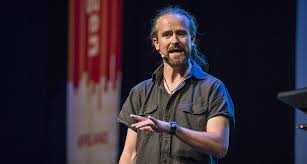
\includegraphics[scale=.6]{images/antonsen2.jpeg}

\intens{{Roger Antonsen}} \\
Universitatea din Oslo

\medskip
TED Talk: Math is the hidden secret to understanding the world

\medskip
\intens{"... înțelegerea constă în abilitatea de a-ți schimba perspectiva"}

\medskip
{\footnotesize \url{https://www.ted.com/talks/roger_antonsen_math_is_the_hidden_secret_to_understanding_the_world}}
\end{center}
\end{frame}
%-------------------------------------------------------

%-------------------------------------------------------
\begin{frame}[fragile]{Un program simplu în  Haskell}

\begin{columns}
\begin{column}{0.55\textwidth}
\begin{lstlisting}[language=Haskell]
data Point = Point Int Int

makePoint :: Int -> Int -> Point
makePoint x y = Point x y

getX :: Point -> Int
getX (Point x y) = x

getY :: Point -> Int
getY (Point x y) = y

origin :: Point
origin = makePoint 0 0
\end{lstlisting}

\end{column}
\begin{column}{0.43\textwidth}
\end{column}
\end{columns}
\end{frame}
%-------------------------------------------------------


%-------------------------------------------------------
\begin{frame}[fragile]{Un program simplu în  Haskell}

\vspace{-.2cm}
\intens{Hai să schimbăm perspectiva!}

\medskip
\begin{columns}
\begin{column}{0.55\textwidth}
\begin{lstlisting}[basicstyle=\small,language=Haskell]
data Point = Point Int Int

makePoint :: Int -> Int -> Point
makePoint x y = Point x y
\end{lstlisting}
\end{column}
\begin{column}{0.4\textwidth}
\[
\infer[\onslide<1>{(Point_I)}]
	{{\color{True}makePoint\ x\ y} : \sel{Point}}
	{{\color{True}x} : \sel{Int} \quad {\color{True}y} : \sel{Int}}
\]
\end{column}
\end{columns}



\begin{columns}
\begin{column}{0.55\textwidth}
\begin{lstlisting}[basicstyle=\small,language=Haskell]
getX :: Point -> Int
getX (Point x y) = x
\end{lstlisting}
\end{column}
\begin{column}{0.4\textwidth}
\[
\infer[\onslide<1>{(Point_{E_1})}]
	{{\color{True}getX\ p} : \sel{Int}}
	{{\color{True}p} : \sel{Point}}
\]
\end{column}
\end{columns}



\begin{columns}
\begin{column}{0.55\textwidth}
\begin{lstlisting}[basicstyle=\small,language=Haskell]
getY :: Point -> Int
getY (Point x y) = y
\end{lstlisting}
\end{column}
\begin{column}{0.4\textwidth}
\[
\infer[\onslide<1>{(Point_{E_2})}]
	{{\color{True}getY\ p} : \sel{Int}}
	{{\color{True}p} : \sel{Point}}
\]
\end{column}
\end{columns}
\end{frame}
%-------------------------------------------------------

%-------------------------------------------------------
\begin{frame}{Generalizare}

\begin{columns}
\begin{column}{0.3\textwidth}
\[
\infer[(Point_I)]
	{{\color{True}makePoint\ x\ y} : \sel{Point}}
	{{\color{True}x} : \sel{Int} \quad {\color{True}y} : \sel{Int}}
\]
\end{column}
\begin{column}{0.1\textwidth}
\end{column}
\begin{column}{0.3\textwidth}
\[
\infer[(\times_I)]
	{{\color{True}\langle M,N \rangle} : \sel{\sigma \times \tau}}
	{{\color{True}M} : \sel{\sigma} \quad {\color{True}N} : \sel{\tau}}
\]
\end{column}
\end{columns}

 \vspace{.6cm}

\begin{columns}
\begin{column}{0.3\textwidth}
\[\quad \quad
\infer[(Point_{E_1})]
	{{\color{True}getX\ p} : \sel{Int}}
	{{\color{True}p} : \sel{Point}}
\]
\end{column}
\begin{column}{0.1\textwidth}
\end{column}
\begin{column}{0.3\textwidth}
\[
\infer[(\times_{E_1})]
	{{\color{True}fst\ M} : \sel{\sigma}}
	{{\color{True}M} : \sel{\sigma \times \tau}}
\]
\end{column}
\end{columns}

 \vspace{.6cm}

\begin{columns}
\begin{column}{0.3\textwidth}
\[\quad \quad
\infer[(Point_{E_2})]
	{{\color{True}getY\ p} : \sel{Int}}
	{{\color{True}p} : \sel{Point}}
\]
\end{column}
\begin{column}{0.1\textwidth}
\end{column}
\begin{column}{0.3\textwidth}
\[
\infer[(\times_{E_2})]
	{{\color{True}snd\ M} : \sel{\tau}}
	{{\color{True}M} : \sel{\sigma \times \tau}}
\]
\end{column}

\end{columns}


\end{frame}
%-------------------------------------------------------

%-------------------------------------------------------
\begin{frame}{Generalizare}

\begin{columns}
\begin{column}{0.3\textwidth}
\[
\infer[(Point_I)]
	{{\color{True}makePoint\ x\ y} : \sel{Point}}
	{{\color{True}x} : \sel{Int} \quad {\color{True}y} : \sel{Int}}
\]
\end{column}
\begin{column}{0.1\textwidth}
\end{column}
\begin{column}{0.3\textwidth}
\[
\infer[(\times_I)]
	{\Gamma \vdash{\color{True}\langle M,N \rangle} : \sel{\sigma \times \tau}}
	{\Gamma \vdash{\color{True}M} : \sel{\sigma} \quad \Gamma \vdash {\color{True}N} : \sel{\tau}}
\]
\end{column}
\end{columns}

 \vspace{.6cm}

\begin{columns}
\begin{column}{0.3\textwidth}
\[\quad \quad
\infer[(Point_{E_1})]
	{{\color{True}getX\ M} : \sel{Int}}
	{{\color{True}M} : \sel{Point}}
\]
\end{column}
\begin{column}{0.1\textwidth}
\end{column}
\begin{column}{0.3\textwidth}
\[
\infer[(\times_{E_1})]
	{\Gamma \vdash{\color{True}fst\ M} : \sel{\sigma}}
	{\Gamma \vdash{\color{True}M} : \sel{\sigma \times \tau}}
\]
\end{column}
\end{columns}

 \vspace{.6cm}

\begin{columns}
\begin{column}{0.3\textwidth}
\[\quad \quad
\infer[(Point_{E_2})]
	{{\color{True}getY\ M} : \sel{Int}}
	{{\color{True}M} : \sel{Point}}
\]
\end{column}
\begin{column}{0.1\textwidth}
\end{column}
\begin{column}{0.3\textwidth}
\[
\infer[(\times_{E_2})]
	{\Gamma \vdash{\color{True}snd\ M} : \sel{\tau}}
	{\Gamma \vdash{\color{True}M} : \sel{\sigma \times \tau}}
\]
\end{column}

\end{columns}


\end{frame}
%-------------------------------------------------------

%-------------------------------------------------------
\begin{frame}[fragile]{Alt exemplu simplu}

\begin{columns}
\begin{column}{0.65\textwidth}
\begin{lstlisting}[language=Haskell]
f = (\x -> x * 3) :: Int -> Int
\end{lstlisting}
\end{column}

\begin{column}{0.4\textwidth}
\[
\infer[\onslide<1>{(fun_I)}]
	{{\color{True}\lambda x.x * 3} : \sel{Int \to Int}}
	{
	\{{\color{True}x} : \sel{Int}\} \vdash {\color{True}x * 3} : \sel{Int} 
	}
\]
%\[
%\infer[\onslide<1>{(fun_I)}]
%	{{\color{True}\lambda x.x * 3} : \sel{Int \to Int}}
%	{
%	\begin{array}{c}
%	\quad\ \ [{\color{True}x} : \sel{Int}] \\
%	\vdots\\
%	{\color{True}x * 3} : \sel{Int} \\
%	\end{array}
%	}
%\]
\end{column}
\end{columns}

 \vspace{.6cm}

\begin{columns}
\begin{column}{0.65\textwidth}
\begin{lstlisting}[language=Haskell]
> f 5
15
\end{lstlisting}
\end{column}

\begin{column}{0.4\textwidth}
\[
\infer[\onslide<1>{(fun_E)}]
	{{\color{True}f\ 5} : \sel{Int}}
	{{\color{True}f} : \sel{Int \to Int} \quad {\color{True}5} : \sel{Int}}
\]
\end{column}
\end{columns}

\end{frame}
%-------------------------------------------------------

%-------------------------------------------------------
\begin{frame}{Generalizare}

\begin{columns}
\begin{column}{0.4\textwidth}
\vspace{-.4cm}
\[
\infer[\onslide<1>{(fun_I)}]
	{{\color{True}\lambda x.x * 3} : \sel{Int \to Int}}
	{
	\{{\color{True}x} : \sel{Int}\} \vdash {\color{True}x * 3} : \sel{Int} 
	}
 \vspace{.35cm}
\]
\end{column}
\begin{column}{0.4\textwidth}
\[
\infer[(\to_{I})]
	{{\color{True}\lambda x.M} : \sel{\sigma \to \tau}}
	{
	\begin{array}{c}
	\{{\color{True}x} : \sel{\sigma}\} \vdash {\color{True}M} : \sel{\tau} \\
	\end{array}
	}
\]
\end{column}
\end{columns}

 \vspace{.6cm}

\begin{columns}
\begin{column}{0.4\textwidth}
\vspace{-.4cm}
\[
\infer[(fun_E)]
	{{\color{True}f\ 5} : \sel{Int}}
	{{\color{True}f} : \sel{Int \to Int} \quad {\color{True}5} : \sel{Int}}
\]
\end{column}
\begin{column}{0.4\textwidth}
\[
\infer[(\to_E)]
	{{\color{True}\app{M}{N}} : \sel{\tau}}
	{{\color{True}M} : \sel{\sigma \to \tau} \quad {\color{True}N} : \sel{\sigma}}
\]
\end{column}
\end{columns}

\end{frame}
%-------------------------------------------------------

%-------------------------------------------------------
\begin{frame}{Generalizare}

\begin{columns}
\begin{column}{0.4\textwidth}
\vspace{-.4cm}
\[
\infer[\onslide<1>{(fun_I)}]
	{{\color{True}\lambda x.x * 3} : \sel{Int \to Int}}
	{
	\{{\color{True}x} : \sel{Int}\} \vdash {\color{True}x * 3} : \sel{Int} 
	}
 \vspace{.35cm}
\]
\end{column}
\begin{column}{0.4\textwidth}
\[
\infer[(\to_{I})]
	{\Gamma \vdash{\color{True}\lambda x.M} : \sel{\sigma \to \tau}}
	{
	\begin{array}{c}
	\Gamma \cup \{{\color{True}x} : \sel{\sigma}\} \vdash {\color{True}M} : \sel{\tau} \\
	\end{array}
	}
\]
\end{column}
\end{columns}

 \vspace{.6cm}

\begin{columns}
\begin{column}{0.4\textwidth}
\vspace{-.4cm}
\[
\infer[(fun_E)]
	{{\color{True}f\ 5} : \sel{Int}}
	{{\color{True}f} : \sel{Int \to Int} \quad {\color{True}5} : \sel{Int}}
\]
\end{column}
\begin{column}{0.4\textwidth}
\[
\infer[(\to_E)]
	{\Gamma \vdash{\color{True}\app{M}{N}} : \sel{\tau}}
	{\Gamma \vdash{\color{True}M} : \sel{\sigma \to \tau} \quad \Gamma \vdash{\color{True}N} : \sel{\sigma}}
\]
\end{column}
\end{columns}

\end{frame}
%-------------------------------------------------------

%-------------------------------------------------------
\begin{frame}{Logica. Ce este adevăt și ce este fals?}
\vspace{-.2cm}

\intens{Hai să schimbăm perspectiva iar!}

\pause
\begin{center}
\intens{Dacă afară este întuneric atunci, \\dacă porcii zboară atunci este întuneric afară.}


\bigskip
\begin{tabular}{rclc}
${\color{True}\sigma}$ & $=$ & {\color{True}afară este întuneric} & \multirow{2}{*}{\hspace{0.5cm} ${\color{True}\sigma} \supset ({\color{True}\tau} \supset {\color{True}\sigma})$} \\
${\color{True}\tau}$ & $=$ & {\color{True}porcii zboară}  \\
\end{tabular}

\pause \bigskip
\intens{Este adevărată această afirmație?} {\color{True} Da!}

 \bigskip
$
\begin{tabular}{c|c|c|c}
\hline
$\sigma$ & $\tau$ & $\tau \supset \sigma$ & $\sigma \supset (\tau \supset \sigma)$ \\
\hline
false & false & {true} & {true} \\  
false & true & false & true \\ 
true & false & true & true \\ 
true & true & true & true
\end{tabular}
$
\end{center}
\end{frame}
%-------------------------------------------------------

%-------------------------------------------------------
\begin{frame}{Semantica unei logici}

Dăm valori variabilelor în mulțimea $\{0,1\}$,\\  \alert{definim o evaluare $e : V \to \{0,1\}$}.

\medskip
Putem să o extindem o evaluare la formule:
\begin{center}
\begin{tabular}{ccc}
$\wedge:\{0,1\}\times \{0,1\}\to\{0,1\}$  & & $\supset:\{0,1\}\times \{0,1\}\to\{0,1\}$\\[.4em]
$
\begin{array}{c|c|c}
\sigma&\tau&  \sigma \wedge \tau  \\ \hline
0 & 0 & 0 \\
0& 1& 0\\
1&0& 0\\
1&1& 1
\end{array} 
$
& &
$
\begin{array}{c|c|c}
\sigma&\tau&  \sigma \supset \tau  \\ \hline
0 & 0 & 1 \\
0& 1& 1\\
1&0& 0\\
1&1& 1
\end{array}
$
\end{tabular}
\end{center}

\medskip 
Dacă pentru toate evaluările posibile, o formulă are valoarea  $1$, atunci spunem că este o \alert{tautologie}.
\end{frame}
%-------------------------------------------------------

%-------------------------------------------------------
\begin{frame}{Sintaxa unei logici}

Dăm metode pentru a manipula simbolurile din logică (i.e., $\supset$, $\wedge$) pentru a stabili când o formulă este \alert{demonstrabilă/teoremă} .

\begin{center}
\begin{tabular}{rcl}
\textbf{\alert{Corectitudine}} & = & sintaxa implică semantica \\
\textbf{\alert{Completitudine}} & = & sintaxa și semantica coincid 
\end{tabular}
\end{center}
\end{frame}
%-------------------------------------------------------

%%-------------------------------------------------------
%\begin{frame}{Un sistem de deducție naturală}
%
%Reguli pentru a manevra fiecare conector logic \\(introducerea si eliminarea conectorilor).
%
%\medskip
%{\footnotesize
%\begin{columns}
%\begin{column}{0.2\textwidth}
%\onslide<1->{
%\[
%\infer[(\wedge_I)]
%	{\sel{A \wedge B}}
%	{\sel{A} \quad \sel{B}}
%\]
%}
%\end{column}
%\begin{column}{0.2\textwidth}
%\onslide<1->{
%\[
%\infer[(\wedge_{E_1})]
%	{\sel{A}}
%	{\sel{A \wedge B}}
%\]
%}
%\end{column}
%\begin{column}{0.2\textwidth}
%\onslide<1->{
%\[
%\infer[(\wedge_{E_2})]
%	{\sel{B}}
%	{\sel{A \wedge B}}
%\]
%}
%\end{column}
%\begin{column}{0.2\textwidth}
%\onslide<1->{
%\[
%\infer[(\supset_{I})]
%	{\sel{A \supset B}}
%	{
%	\begin{array}{c}
%	 [\sel{A}] \\
%	\vdots\\
%	 \sel{B} \\
%	\end{array}
%	}
%\]
%}
%\end{column}
%\begin{column}{0.2\textwidth}
%\onslide<1->{
%\[
%\infer[(\supset_E)]
%	{\sel{B}}
%	{\sel{A \supset B} \quad \sel{A}}
%\]
%}
%\end{column}
%\end{columns}
%}
%
%%{\color{True} Exemplu.}
%%\[
%%\infer[(\wedge_I)]
%%	{q \wedge r}
%%	{
%%	\infer[(\wedge_{e_2})]{q}{p\wedge q} & r
%%	}
%%\]
%
%
%
%\end{frame}
%%-------------------------------------------------------

%-------------------------------------------------------
\begin{frame}{Un sistem de deducție naturală}

Reguli pentru a manevra fiecare conector logic \\(introducerea si eliminarea conectorilor).

\begin{columns}
\begin{column}{0.3\textwidth}
\onslide<1->{
\[
\infer[(\wedge_I)]
	{\Gamma \vdash\sel{\sigma \wedge \tau}}
	{\Gamma \vdash\sel{\sigma} \quad \Gamma \vdash\sel{\tau}}
\]
}
\end{column}
\begin{column}{0.3\textwidth}
\onslide<1->{
\[
\infer[(\wedge_{E_1})]
	{\Gamma \vdash\sel{\sigma}}
	{\Gamma \vdash\sel{\sigma \wedge \tau}}
\]
}
\end{column}
\begin{column}{0.3\textwidth}
\onslide<1->{
\[
\infer[(\wedge_{E_2})]
	{\Gamma \vdash\sel{\tau}}
	{\Gamma \vdash\sel{\sigma \wedge \tau}}
\]
}
\end{column}
\end{columns}

\begin{columns}
\begin{column}{0.4\textwidth}
\onslide<1->{
\[
\infer[(\supset_{I})]
	{\Gamma \vdash\sel{\sigma \supset \tau}}
	{
	\Gamma \cup \{\sel{\sigma}\} \vdash \sel{\tau} 
	}
\]
}
\end{column}
\begin{column}{0.4\textwidth}
\onslide<1->{
\[
\infer[(\supset_E)]
	{\Gamma \vdash\sel{\tau}}
	{\Gamma \vdash\sel{\sigma \supset \tau} \quad \Gamma \vdash \sel{\sigma}}
\]
}
\end{column}
\end{columns}


\vspace{-.4cm}
\begin{center}
\onslide<1->{\intens{Arată cunoscut?}}
\end{center}

\end{frame}
%-------------------------------------------------------

%-------------------------------------------------------
\begin{frame}{Corespondența Curry-Howard}

\begin{center}
\begin{tabular}{cc}
\intens{$\lambda$-calcul cu tipuri}  & \intens{Deducție naturală}
\\  [.2cm] 
\infer[(\times_I)]
	{\Gamma \vdash{\color{True}\langle M,N \rangle} : \sel{\sigma \times \tau}}
	{\Gamma \vdash{\color{True}M} : \sel{\sigma} \quad \Gamma \vdash {\color{True}N} : \sel{\tau}}
&
\infer[(\wedge_I)]
	{\Gamma \vdash\sel{\sigma \wedge \tau}}
	{\Gamma \vdash\sel{\sigma} \quad \Gamma \vdash \sel{\tau}}
\\ [.3cm]
\infer[(\times_{E_1})]
	{\Gamma \vdash{\color{True}fst\ M} : \sel{\sigma}}
	{\Gamma \vdash{\color{True}M} : \sel{\sigma \times \tau}}
&
\infer[(\wedge_{E_1})]
	{\Gamma \vdash\sel{\sigma}}
	{\Gamma \vdash\sel{\sigma \wedge \tau}}
\\  [.3cm] 
\infer[(\times_{E_2})]
	{\Gamma \vdash{\color{True}snd\ p} : \sel{\tau}}
	{\Gamma \vdash{\color{True}p} : \sel{\sigma \times \tau}}
&
\infer[(\wedge_{E_2})]
	{\Gamma \vdash\sel{\tau}}
	{\Gamma \vdash\sel{\sigma \wedge \tau}}
\\ [.3cm]
\infer[(\to_{I})]
	{\Gamma \vdash{\color{True}\lambda x.M} : \sel{\sigma \to \tau}}
	{
	\begin{array}{c}
	\Gamma \cup \{{\color{True}x} : \sel{\sigma}\} \vdash {\color{True}M} : \sel{\tau} \\
	\end{array}
	}
& 
\infer[(\supset_{I})]
	{\Gamma \vdash\sel{\sigma \supset \tau}}
	{
	\Gamma \cup \{\sel{\sigma}\} \vdash \sel{\tau} 
	}
\\  [.3cm] 
\infer[(\to_E)]
	{\Gamma \vdash{\color{True}\app{M}{N}} : \sel{\tau}}
	{\Gamma \vdash{\color{True}M} : \sel{\sigma \to \tau} \quad \Gamma \vdash{\color{True}N} : \sel{\sigma}}
&
\infer[(\supset_E)]
	{\Gamma \vdash\sel{\tau}}
	{\Gamma \vdash\sel{\sigma \supset \tau} \quad \Gamma \vdash \sel{\sigma}}
 
\end{tabular}

\medskip 
\intens{\textit{Propositions are types! $\heartsuit$} } 
\end{center}

\end{frame}
%-------------------------------------------------------

%
%
%%-------------------------------------------------------
%\begin{frame}{Corespondența Curry-Howard}
%
%\begin{center}
%\begin{tabular}{cc}
%\intens{Un $\lambda$-calcul cu tipuri}  & \intens{Un sistem de deducție naturală}
%\\  [.2cm] 
%$
%\infer[(\times_I)]
%	{{\color{True}\langle a,b \rangle} : \sel{A \times B}}
%	{{\color{True}a} : \sel{A} \quad {\color{True}b} : \sel{B}}
%$
%&
%$
%\infer[(\wedge_I)]
%	{\sel{A \wedge B}}
%	{\sel{A} \quad \sel{B}}
%$
%\\ [.3cm]
%$
%\infer[(\times_{E_1})]
%	{{\color{True}fst\ p} : \sel{A}}
%	{{\color{True}p} : \sel{A \times B}}
%$
%&
%$
%\infer[(\wedge_{E_1})]
%	{\sel{A}}
%	{\sel{A \wedge B}}
%$
%\\  [.3cm] 
%$
%\infer[(\times_{E_2})]
%	{{\color{True}snd\ p} : \sel{B}}
%	{{\color{True}p} : \sel{A \times B}}
%$
%&
%$
%\infer[(\wedge_{E_2})]
%	{\sel{B}}
%	{\sel{A \wedge B}}
%$
%\\ [.3cm]
%
%$
%\infer[(\to_{I})]
%	{{\color{True}\lambda x.n} : \sel{A \to B}}
%	{
%	\begin{array}{c}
%	 [{\color{True}x} : \sel{A}] \\
%	\vdots\\
%	{\color{True}b} : \sel{B} \\
%	\end{array}
%	}
%$
%& 
%$
%\infer[(\supset_{I})]
%	{\sel{A \supset B}}
%	{
%	\begin{array}{c}
%	 [\sel{A}] \\
%	\vdots\\
%	 \sel{B} \\
%	\end{array}
%	}
%$
%\\  [.3cm] 
%$
%\infer[(\to_E)]
%	{{\color{True}f\ x} : \sel{B}}
%	{{\color{True}f} : \sel{A \to B} \quad {\color{True}x} : \sel{A}}
%$
%&
%$
%\infer[(\supset_E)]
%	{\sel{B}}
%	{\sel{A \supset B} \quad \sel{A}}
%$ 
%\end{tabular}
%
%\medskip 
%\textit{{\color{True}Propositions are types! $\heartsuit$} } 
%\end{center}
%
%\end{frame}
%%-------------------------------------------------------
%
%-------------------------------------------------------
\begin{frame}{Să analizăm mai atent}

\begin{center}
\begin{tabular}{cc}
\intens{$\lambda$-calcul cu tipuri}  & \intens{Deducție naturală} \\
$\Gamma \vdash \type{M}{\sigma}$
& 
$\Gamma \vdash \sel{\sigma}$
\end{tabular}

\vspace{.6cm} 
\intens{Faptul că există un termen de tip $\sigma$ \textit{(inhabitation of type $\sigma$)} \\
înseamnă că $\sigma$ este teoremă/are o demonstrație în logică! $\heartsuit$}

\end{center}

\end{frame}
%-------------------------------------------------------

%-------------------------------------------------------
\begin{frame}{Să analizăm mai atent}

\vspace{-.6cm}
\begin{center}
\begin{tabular}{ccc}
\intens{$\lambda$-calcul cu tipuri}  & & \intens{Deducție naturală}
\\  [.2cm] 
\infer[(\to_I)]
	{\vdash \type{\abs{x}{x}}{\sigma \to \sigma}}
	{
	 \{\type{x}{\sigma}\} \vdash \type{x}{\sel{\sigma}}
	}
 & &
$
\infer[(\supset_I)]
	{\onslide<1->{\vdash\sel{\sigma \supset \sigma}}}
	{
	\begin{array}{c}
	 \{\sel{\sigma}\} \vdash \sel{\sigma}
	\end{array}
	}
$
\\  [.6cm]  \pause
\infer[(\to_I)]
	{\vdash \type{\abs{x}{(\abs{y}{x})}}{\sigma \to (\tau \to \sigma)}}
	{
	\infer[(\to_I)]
	{\{\type{x}{\sigma}\} \vdash \type{\abs{y}{x}}{\tau \to \sigma}}
	{
	 \infer
		{\{\type{x}{\sigma}, \type{y}{\tau}\} \vdash \type{x}{\sigma}}
		{}
	}
}
& &
\infer[(\supset_I)]
	{\vdash {\sel{\sigma \to (\tau \to \sigma)}}}
	{
	\infer[(\supset_I)]
	{\{\sel{\sigma}\} \vdash \sel{\tau \to \sigma}}
	{
	 \infer
		{\{ \sel{\sigma}, \sel{\tau}\} \vdash \sel{\sigma}}
		{}
	}
}
\end{tabular}

\vspace{.4cm} \pause
{\intens{Proofs are Terms! $\heartsuit$}}

{Demonstrațiile sunt termeni!}
\end{center}

\end{frame}
%-------------------------------------------------------


\renewcommand{\arraystretch}{1.3}

%-------------------------------------------------------
\begin{frame}{Corespondența Curry-Howard}

\begin{center}
\begin{tabular}{ccc}
 \hline 
\intens{Teoria Tipurilor} & & \intens{Logică}  \\  \hline 
tipuri & &  formule\\
termeni & &  demonstrații\\
\textit{inhabitation} a tipului $\sigma$ & & demonstrație a lui $\sigma$\\
  \hline   \pause 
tip produs  & &  conjuncție\\ 
tip funcție & & implicație  \\ \pause
tip sumă   & &  disjuncție\\ 
tipul void  & &  false \\
tipul unit  & & true \\ \hline
\end{tabular}
\end{center}
\end{frame}
%-------------------------------------------------------



\renewcommand{\arraystretch}{1}

%-------------------------------------------------------
\begin{frame}{Logica intuiționistă}

\begin{itemize}
	\item Logică \alert{constructivistă}
	\medskip
	\item Bazată pe noțiunea de \alert{demonstrație}
	\medskip
	\item Utilă deoarece demonstrațiile \alert{sunt executabile} și \alert{produc exemple}

	Permite "extragererea" de programe demonstrate a fi corecte.
	\medskip
	\item Baza pentru \textit{proof assistants} (e.g., Coq, Agda, Idris)
	\medskip 
	\item {\color{red} Următoarele formule echivalente nu sunt demonstrabile în logica intuiționistă!} 
	\begin{itemize}
		\item dubla negație: $\neg \neg \varphi \supset \varphi$ \quad 
		\item excluded middle: $\varphi \vee \neg \varphi$ 
		\item legea lui Pierce: $((\varphi \supset \tau) \supset \varphi) \supset \varphi$ 
	\end{itemize}
	\medskip 
	\item {\color{red} Nu există semantică cu tabele de adevăr pentru logica intuiționistă!} 
		Semantici alternative (e.g., semantica de tip Kripke)
\end{itemize}
\end{frame}

%-------------------------------------------------------
\begin{frame}{Corespondența Curry-Howard}

Inițial, corespondența Curry-Howard a fost între
\begin{center}
\begin{tabular}{ccc}
\intens{Calculul } & &  \intens{Sistemul de deducție naturală}\\
\intens{Church $\lambda\to$} & & \intens{al lui Gentzen pentru}\\
& & \intens{logica intuiționistă}
\end{tabular}
\end{center}
\end{frame}
%-------------------------------------------------------


\renewcommand{\arraystretch}{1}

%-------------------------------------------------------
\begin{frame}{De ce?}

\begin{itemize}
	\item \intens{Este pur si simplu fascinant}
	\medskip 
	\item \intens{Nu gândiți logica și informatica ca domenii diferite.}
	\medskip 
	\item \intens{Gândind din perspective diferite ne poate ajuta să știm ce este posibil/imposibil.}
	\medskip
	\item \intens{Teoria tipurilor nu ar trebui să fie o adunătură \textit{ad hoc} de reguli!}
\end{itemize}
\end{frame}
%-------------------------------------------------------


%------------------------------------------------
\begin{frame}
  \vfill
  \centering

\textbf{\large \alert{Quiz time!}}


\includegraphics[scale=.35]{../Quiz/C06-Q1.png}

 \url{https://tinyurl.com/C06-Quiz1}
  \vfill
\end{frame}

%---------------------------------------------
\begin{frame}
  \vfill
  \centering

\textbf{Pe săptămâna viitoare!}

  \vfill
\end{frame}
\end{document}







